\section{Proposed Method}

\sectioncover

\subsection{Key idea}

\begin{frame}
    \begin{itemize}
        \item Assumptions:
              \begin{itemize}
                  \item The phase field $d$ has a \textcolor{blue}{compact support} whose width $W$ is known a priori.
                  \item The approximated crack normal $\bfn_d \approx \grad d / \norm{\grad d}$ satisfies \textcolor{blue}{$\divergence \bfn_d \approx 0$}.
              \end{itemize}
        \item In 1D, for any integrable function $f: [a,b] \mapsto \mathbb{R}$, there exists a constant $f^*$ s.t.
              \begin{align*}
                  I = \int_a^b f \diff{s} = f^* (b-a).
              \end{align*}
        \item Next, we introduce an auxliary integrable function $I^*: [a,b] \mapsto \mathbb{R}$ that is continuously differentiable on $(a,b)$, and the constant $I = f^*(b-a)$ can be solved as
              \begin{align*}
                  \int_a^b \left[ (b-a) f - I^* \right] \diff{s} & = 0, \quad \text{subject to } I^*_{,s}(x) = 0 \quad \forall x \in (a,b), \\
                  I^*                                            & = I, \quad \forall x \in [a, b].
              \end{align*}
        \item In 2D and 3D, the problem can be generalized as
              \begin{equation*}
                  \boxed{\int_\Omega \left( W f \bfn - \bfI^* \right) \diff{V} = \bs{0}, \quad \text{subject to } \grad \bfI^* \bfn = \bs{0} \quad \forall \bfx \in \Omega.}
              \end{equation*}
    \end{itemize}
\end{frame}

\subsection{Jump estimation}

\begin{frame}
    \begin{itemize}
        \item The jump at a discontinuity can be expressed using the dirac delta function in the integral form, and can be further regularized by a finite characteristic length.
              \begin{align*}
                  \jump{u} = u^+ - u^- = \int_{0^+}^\infty u \delta_\Gamma \diff{x} - \int_{-\infty}^{0^-} u \delta_\Gamma \diff{x} = \lim_{\epsilon\to 0} \left( \int_{0^+}^\infty u \delta_\Gamma^\epsilon \diff{x} - \int_{-\infty}^{0^-} u \delta_\Gamma^\epsilon \diff{x} \right).
              \end{align*}
        \item In the context of phase field, a family of indicator functions $I(d)$ can be used as such regularization:
              \begin{align*}
                  \jump{u} \approx \int_{0^+}^\infty u \norm{\grad I} \diff{x} - \int_{-\infty}^{0^-} u \norm{\grad I} \diff{x}.
              \end{align*}
        \item Following the remark on the previous page, this directional jump be solved as
              \begin{equation*}
                  \boxed{\int_\Omega \left( W u \bfn - \bfJ_u \right) \diff{V} = \bs{0}, \quad \text{subject to } \grad \bfJ_u \bfn = \bs{0} \quad \forall \bfx \in \Omega,}
              \end{equation*}
              which is the integral statement of
              \begin{align*}
                  \bfJ_u = \jump{u}\bfn, \quad \forall \bfx \in \Omega.
              \end{align*}
    \end{itemize}
\end{frame}

\subsection{Numerical treatments}

\begin{frame}
    \begin{itemize}
        \item The directional jump is solved using FEM. The pathwise-constant constraint can be enforced with a penalty approach:
              \begin{align*}
                  r = \left( W u \bfn - \bfJ_u, \delta \bfJ_u \right) + \alpha \left( \grad \bfJ_u \bfn, \grad \delta\bfJ_u \bfn \right).
              \end{align*}
        \item<4-> The \textcolor{blue}{crack tips} can be \textcolor{blue}{``ignored''} using the so-called crack tip indicator obtained by projecting the phase field onto an anisotropic subspace.
        \item<5-> On unstructured meshes, a better \textcolor{blue}{level-set} can be \textcolor{blue}{reconstructed} using the phase field to yield a more accurate crack normal approximation.
        \item<6-> Some remarks on the computational cost:
            \begin{itemize}
                \item Computing/broadcasting the jump across the phase field crack is now fully \textcolor{blue}{``automated''}, at the cost of solving \textcolor{blue}{one (optionally up to three) additional system of equations}.
                \item The additional auxiliary problems are all \textcolor{blue}{linear}.
                \item The level-set and the crack tip indicator can be solved on a \textcolor{blue}{confined domain} where $d > 0$. The directional jump can be solved on an even smaller domain excluding the crack tips.
            \end{itemize}
        \item<7-> The proposed method \textcolor{blue}{allows for monolithic coupling} between the jump and other physics.
    \end{itemize}
    \vspace{-70pt}
    \only<2>{
        \begin{figure}
            \centering
            \begin{subfigure}{0.32\textwidth}
                \centering
                \caption*{$d$}
                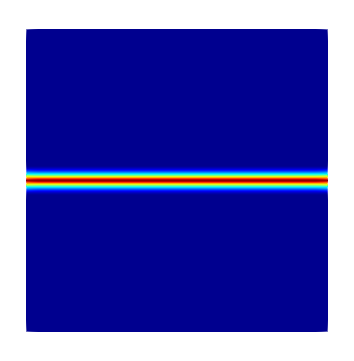
\includegraphics[width=0.6\textwidth]{method/figures/d_1.png}
            \end{subfigure}
            \begin{subfigure}{0.32\textwidth}
                \centering
                \caption*{$u_y$}
                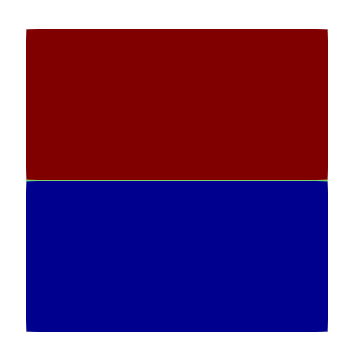
\includegraphics[width=0.6\textwidth]{method/figures/uy_1.png}
            \end{subfigure}
            \begin{subfigure}{0.32\textwidth}
                \centering
                \caption*{$\jump{u_y}$}
                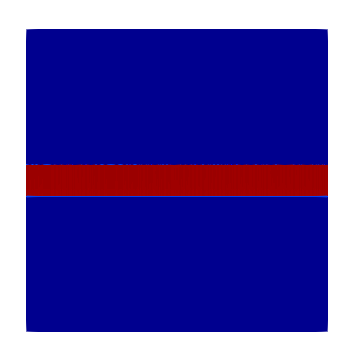
\includegraphics[width=0.6\textwidth]{method/figures/w_1.png}
            \end{subfigure}
            \caption*{It works well for a \textcolor{blue}{fully developed crack}.}
        \end{figure}
    }
    \only<3>{
        \begin{figure}
            \centering
            \begin{subfigure}{0.32\textwidth}
                \centering
                \caption*{$d$}
                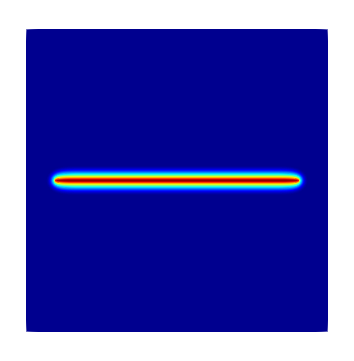
\includegraphics[width=0.6\textwidth]{method/figures/d_0.8.png}
            \end{subfigure}
            \begin{subfigure}{0.32\textwidth}
                \centering
                \caption*{$u_y$}
                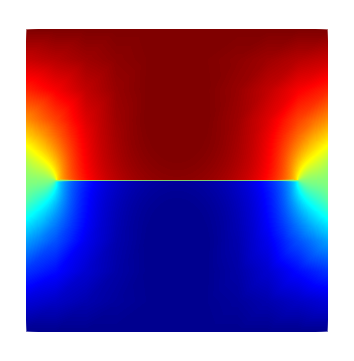
\includegraphics[width=0.6\textwidth]{method/figures/uy_0.8.png}
            \end{subfigure}
            \begin{subfigure}{0.32\textwidth}
                \centering
                \caption*{$\jump{u_y}$}
                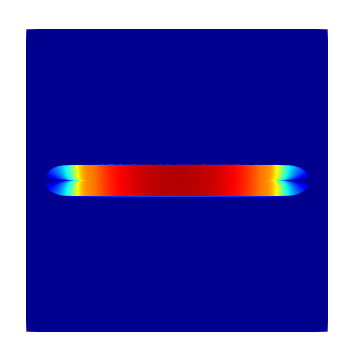
\includegraphics[width=0.6\textwidth]{method/figures/w_0.8_wo_cti.png}
            \end{subfigure}
            \caption*{But it doesn't work well for an \textcolor{blue}{embedded crack}. Recall our assumption $\divergence \bfn \approx 0$.}
        \end{figure}
    }
    \only<4>{
        \begin{figure}
            \centering
            \begin{subfigure}{0.32\textwidth}
                \centering
                \caption*{$d$}
                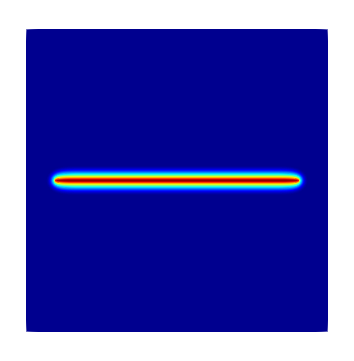
\includegraphics[width=0.6\textwidth]{method/figures/d_0.8.png}
            \end{subfigure}
            \begin{subfigure}{0.32\textwidth}
                \centering
                \caption*{$u_y$}
                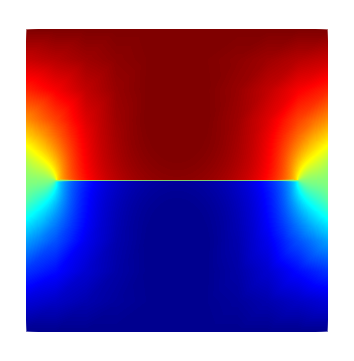
\includegraphics[width=0.6\textwidth]{method/figures/uy_0.8.png}
            \end{subfigure}
            \begin{subfigure}{0.32\textwidth}
                \centering
                \caption*{$\jump{u_y}$}
                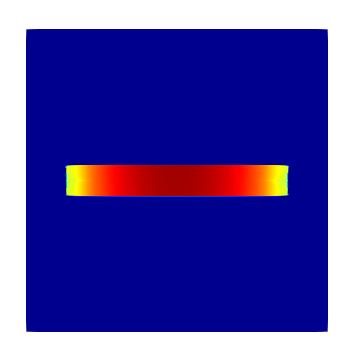
\includegraphics[width=0.6\textwidth]{method/figures/w_0.8_w_cti.png}
            \end{subfigure}
            \caption*{}
        \end{figure}
    }
\end{frame}